\documentclass[11pt]{article}

\usepackage{classDM17}
\usepackage{mathtools}
\DeclarePairedDelimiter\ceil{\lceil}{\rceil}
\DeclarePairedDelimiter\floor{\lfloor}{\rfloor}

\title{Asmt 1: Hash Functions and PAC Algorithms}
\author{Turn in (\textbf{a pdf}) through Canvas by 2:45pm: \\
Wednesday, January 25}
\date{}

\begin{document}
\maketitle






%%%%%%%%%%%%%%%%%%%%%%%%%%%%%%%%%%%%%%%%%%%%%%%%%%%%
%%%%%%%%%%%%%%%%%%%%%%%%%%%%%%%%%%%%%%%%%%%%%%%%%%%%
%%%%%%%%%%%%%%%%%%%%%%%%%%%%%%%%%%%%%%%%%%%%%%%%%%%%
\section*{Overview}

In this assignment you will experiment with random variation over discrete events.  


It will be very helpful to use the analytical results and the experimental results to help verify the other is correct.  If they do not align, you are probably doing something wrong (this is a very powerful and important thing to do whenever working with real data).  


\vspace{.1in}

\emph{As usual, it is highly recommended that you use LaTeX for this assignment.  If you do not, you may lose points if your assignment is difficult to read or hard to follow.  Find a sample form in this directory:
\url{http://www.cs.utah.edu/~jeffp/teaching/latex/}}

%%%%%%%%%%%%%%%%%%%%%%%%%%%%%%%%%%%%%%%%%%%%%%%%%%%%
%%%%%%%%%%%%%%%%%%%%%%%%%%%%%%%%%%%%%%%%%%%%%%%%%%%%
%%%%%%%%%%%%%%%%%%%%%%%%%%%%%%%%%%%%%%%%%%%%%%%%%%%%
\section{Birthday Paradox (30 points)}

Consider a domain of size $n = 4000$.  

\paragraph{A: (5 points)}
Generate random numbers in the domain $[n]$ until two have the same value.  How many random trials did this take?  
We will use $k$ to represent this value. \\

It took me $130$ trials to get a collision. I did not set the seed for the random number generator and so I got a different value for each run. The value of $130$ was for one of the runs.

\paragraph{B: (10 points)}  
Repeat the experiment $m = 300$ times, and record for each time how many random trials this took.  Plot this data as a \emph{cumulative density plot} where the $x$-axis records the number of trials required $k$, and the $y$-axis records the fraction of experiments that succeeded (a collision) after $k$ trials.  The plot should show a curve that starts at a $y$ value of $0$, and increases as $k$ increases, and eventually reaches a $y$ value of $1$.  \\

The cumulative density plot is shown in figure \ref{cumplot1}.

\begin{figure}[!htb]
\centering
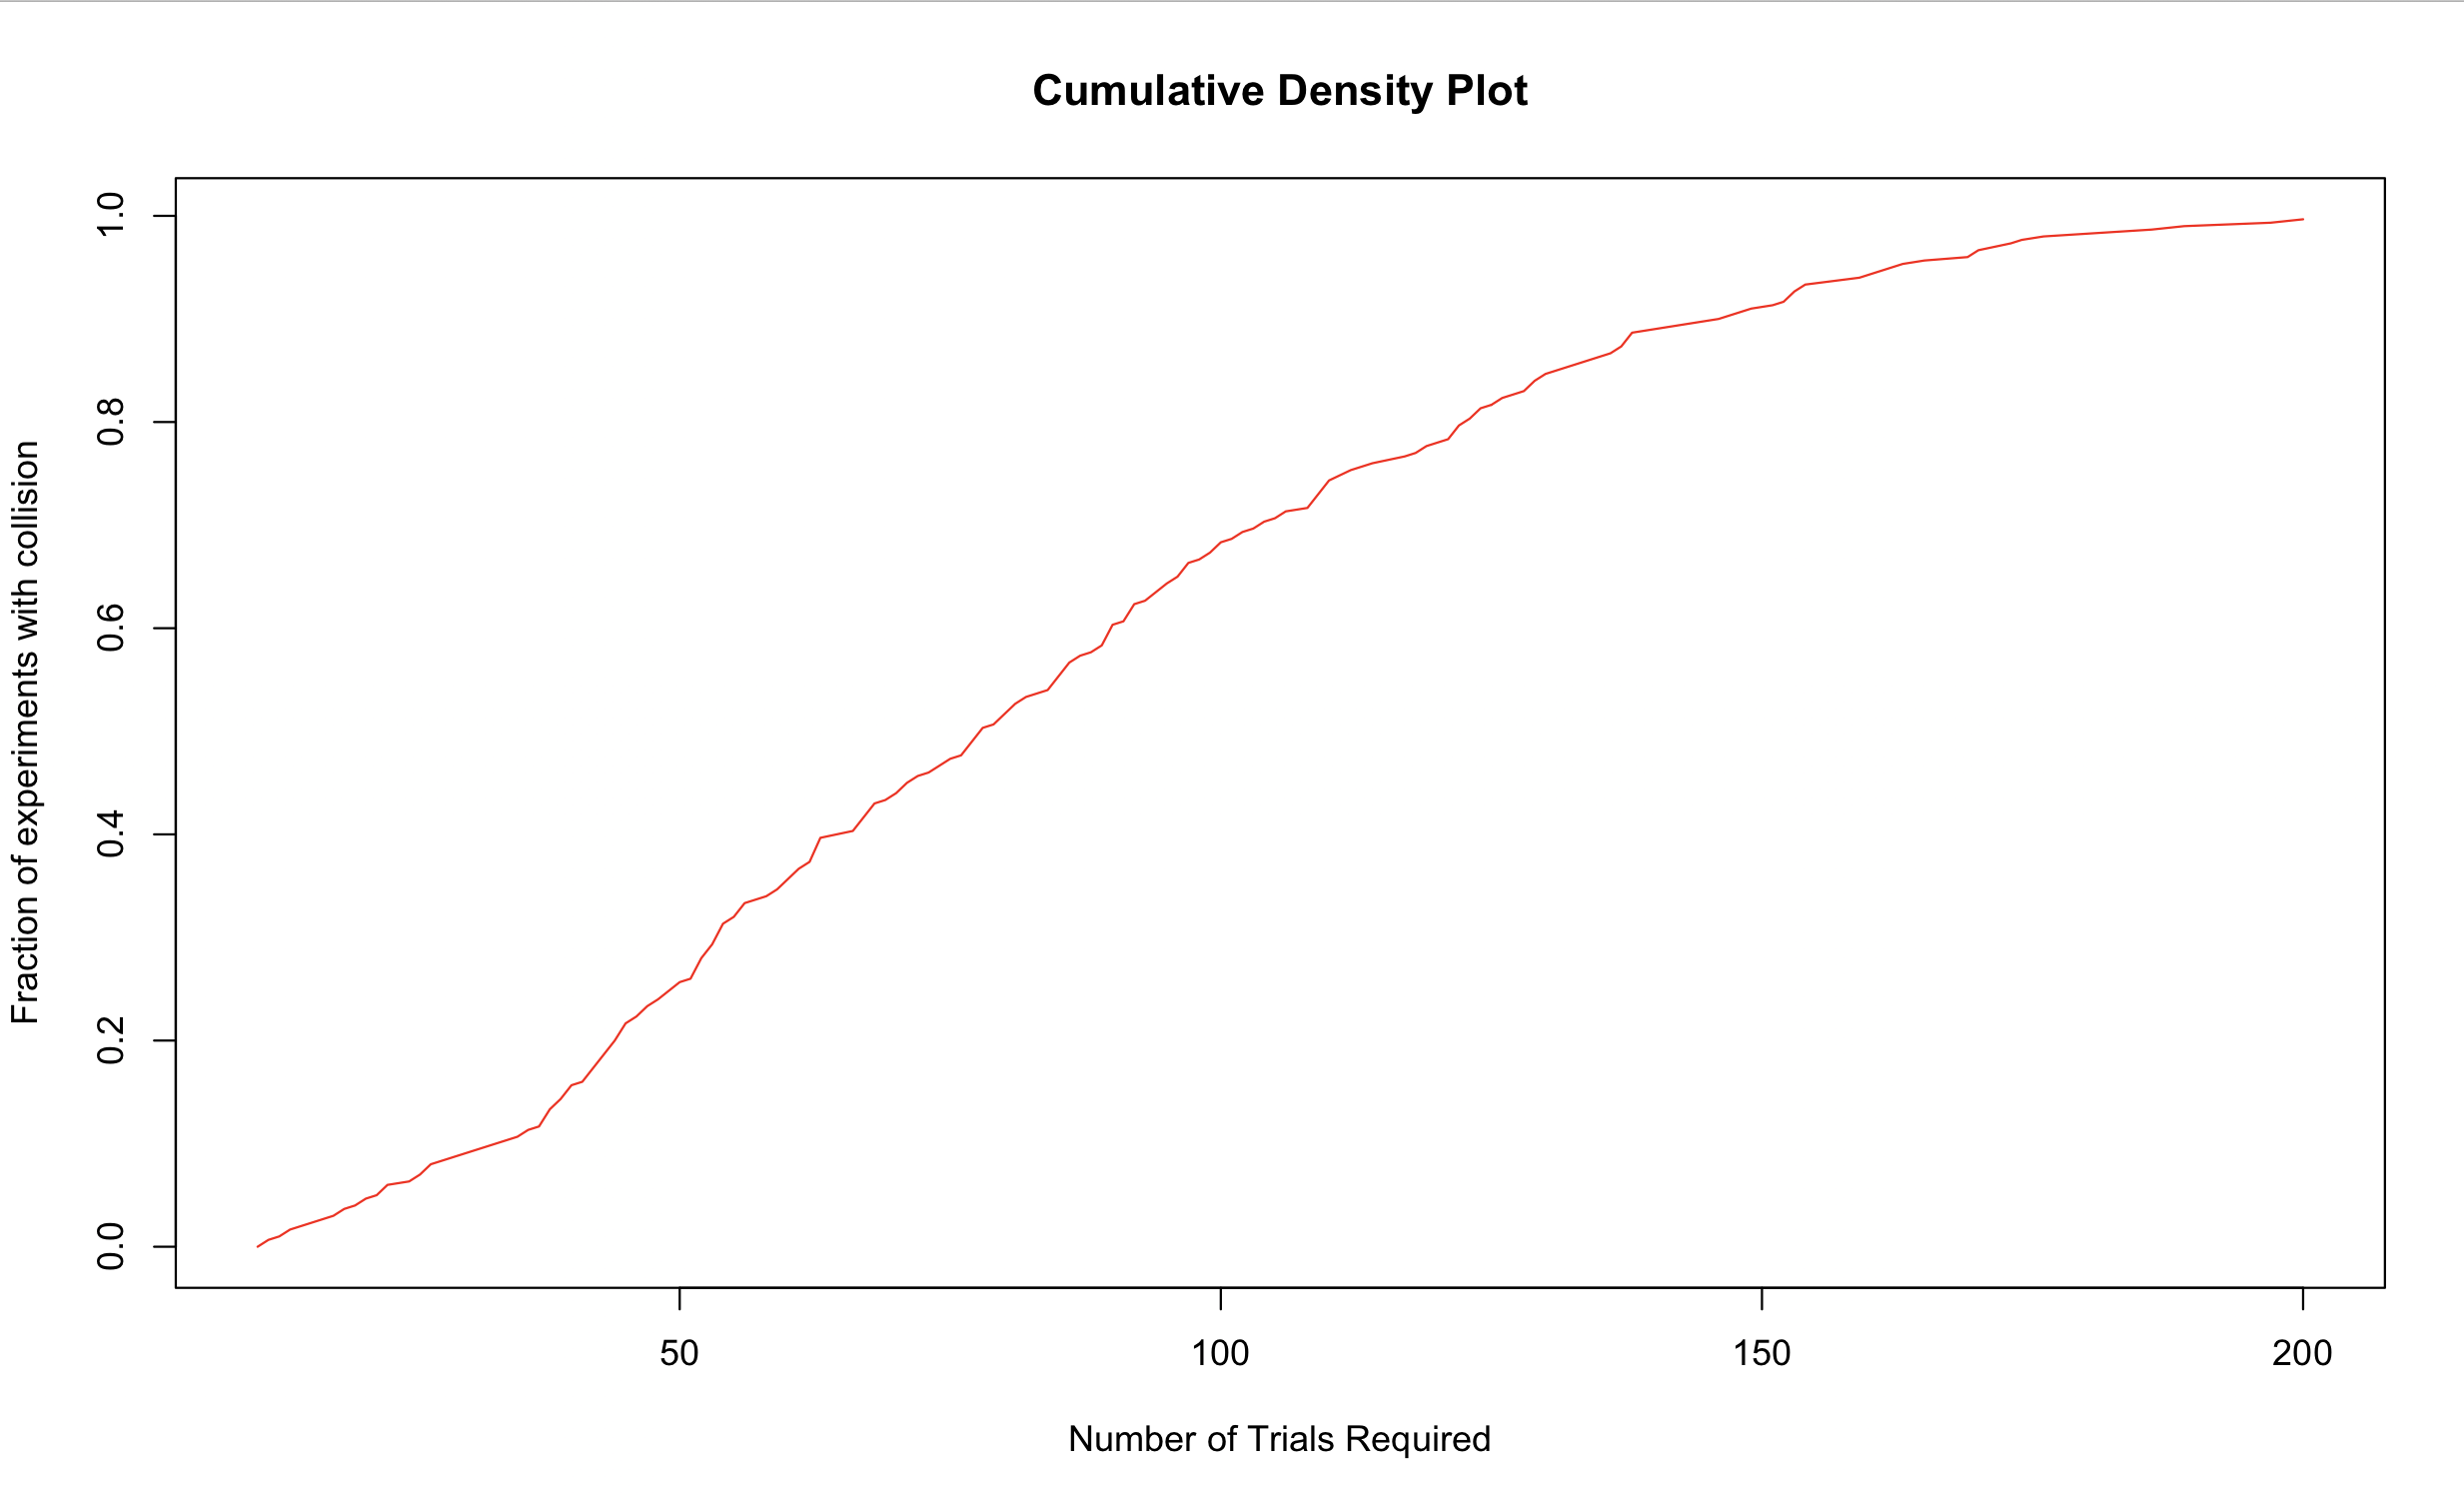
\includegraphics[width=5.5in]{figures/cumdenplot1b.png}
\caption{Cumulative density plot for trials till collision for experiment repeated $300$ times for a domain of size $4000$}
\label{cumplot1}
\end{figure}

\paragraph{C: (5 points)}  
Empirically estimate the expected number of $k$ random trials in order to have a collision.  That is, add up all values $k$, and divide by $m$.  \\

Empirical estimate for the expected number of random trials till collision is $85.9466$.

\paragraph{D: (10 points)}  
Describe how you implemented this experiment and how long it took for $m = 300$ trials.  \\

For each iteration of the experiment where it was run $m$ times, the number of trials till collision was recorded. The trials till collision were put into an array and the array was sorted. For each entry in the array with index $x$, the corresponding fraction of experiments that succeeded in having a collision was computed as $\frac{x}{m}$.\\

For $300$ trials and a domain size of $4000$, it took $29$ $ms$ to run.\\

Show a plot of the run time as you gradually increase the parameters $n$ and $m$.  
(For at least 3 fixed values of $m$ between 300 and 10,000, plot the time as a function of $n$.)
You should be able to reach values of $n = 1{,}000{,}000$ and $m = 10{,}000$.  \\

The run time plot is shown in figure \ref{bpruntimes}.

\begin{figure}[!htb]
\centering
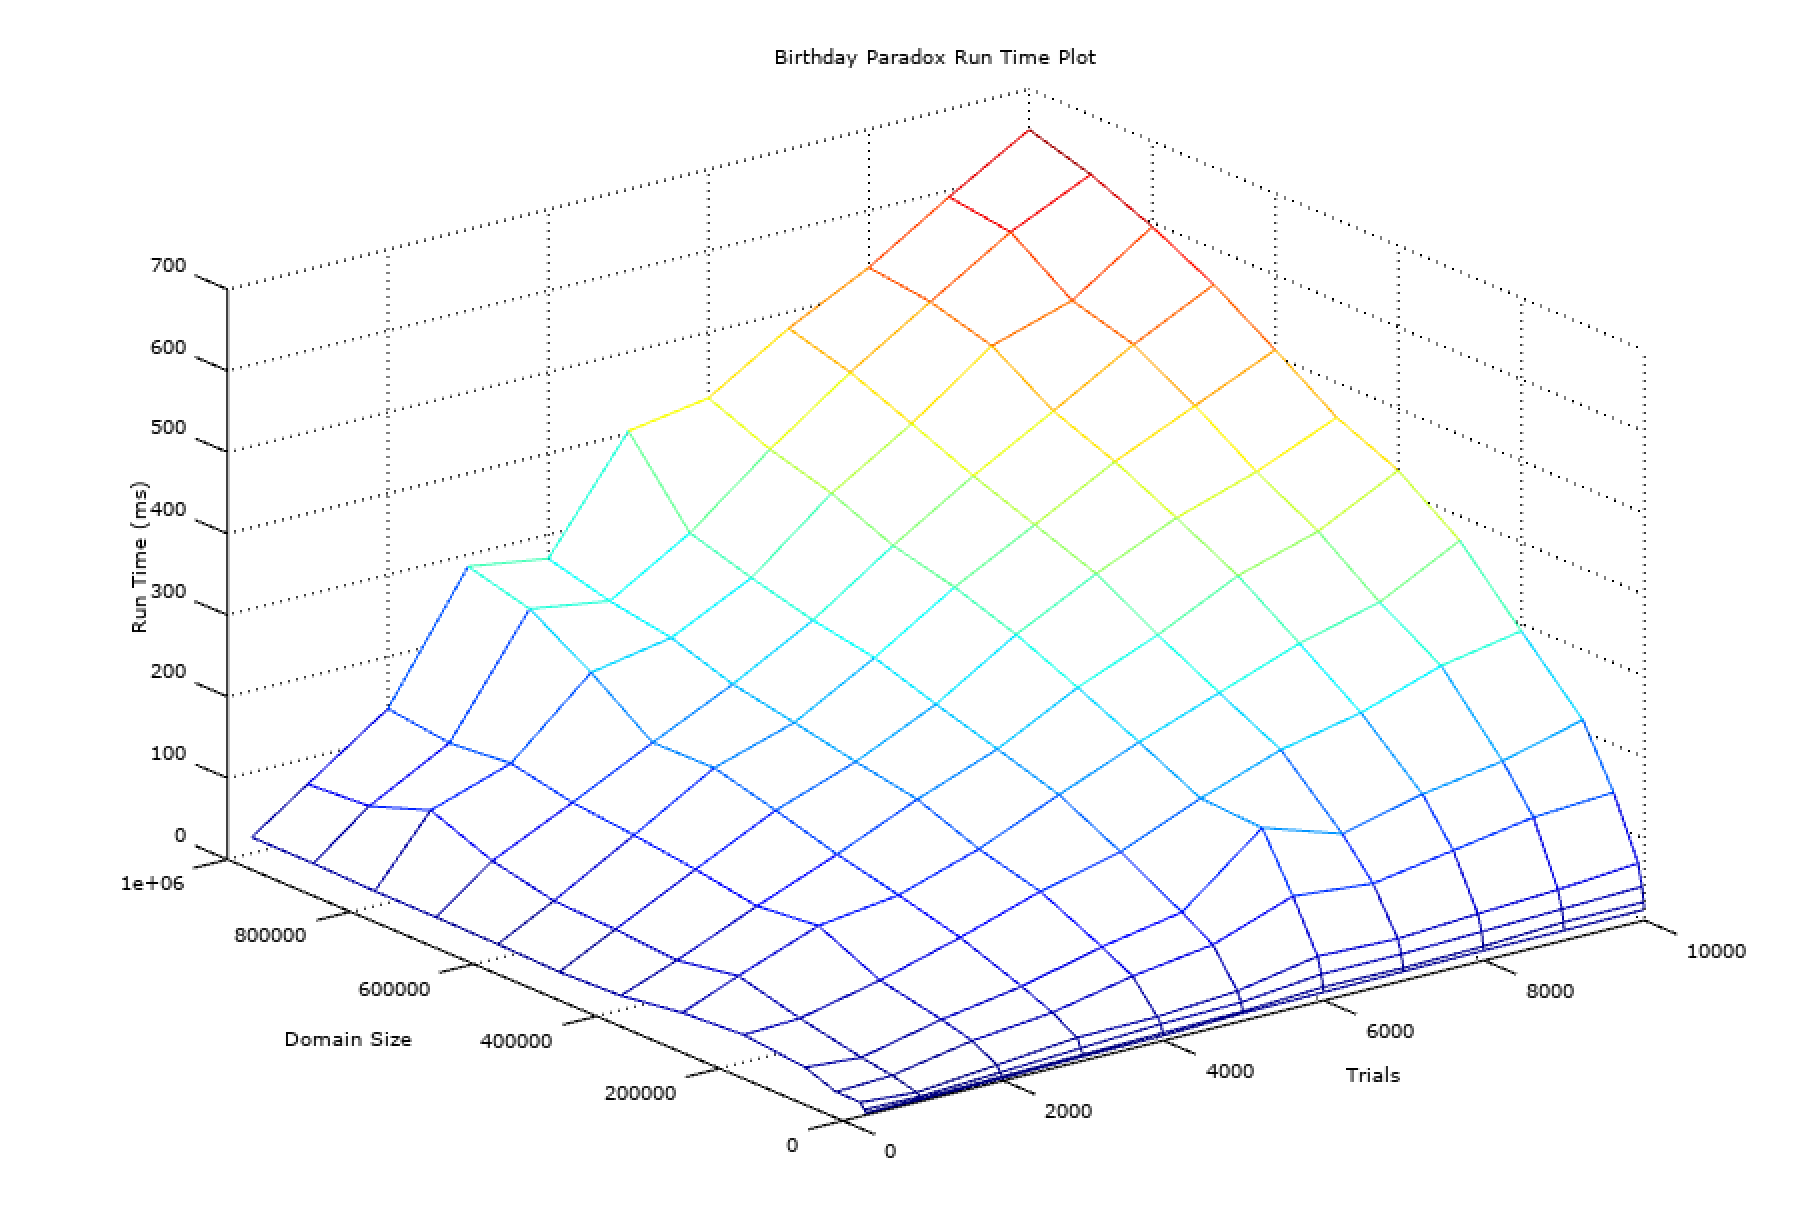
\includegraphics[width=5.5in]{figures/bpruntimes.png}
\caption{Birthday Paradox run time plot}
\label{bpruntimes}
\end{figure}

%%%%%%%%%%%%%%%%%%%%%%%%%%%%%%%%%%%%%%%%%%%%%%%%%%%%
%%%%%%%%%%%%%%%%%%%%%%%%%%%%%%%%%%%%%%%%%%%%%%%%%%%%
%%%%%%%%%%%%%%%%%%%%%%%%%%%%%%%%%%%%%%%%%%%%%%%%%%%%
\section{Coupon Collectors (30 points)}

Consider a domain $[n]$ of size $n = 200$.  

\paragraph{A: (5 points)}
Generate random numbers in the domain $[n]$ until every value $i \in [n]$ has had one random number equal to $i$.
How many random trials did this take?  
We will use $k$ to represent this value.  \\

It took $1434$ random trials for generating all numbers up to $200$.

\paragraph{B: (10 points)}
Repeat step $A$ for $m=300$ times, and for each repetition record the value $k$ of how many random trials we required to collect all values $i \in [n]$.  
Make a cumulative density plot as in 1.B.  \\

The cumulative density plot is shown in figure \ref{cumplot2}.

\begin{figure}[!htb]
\centering
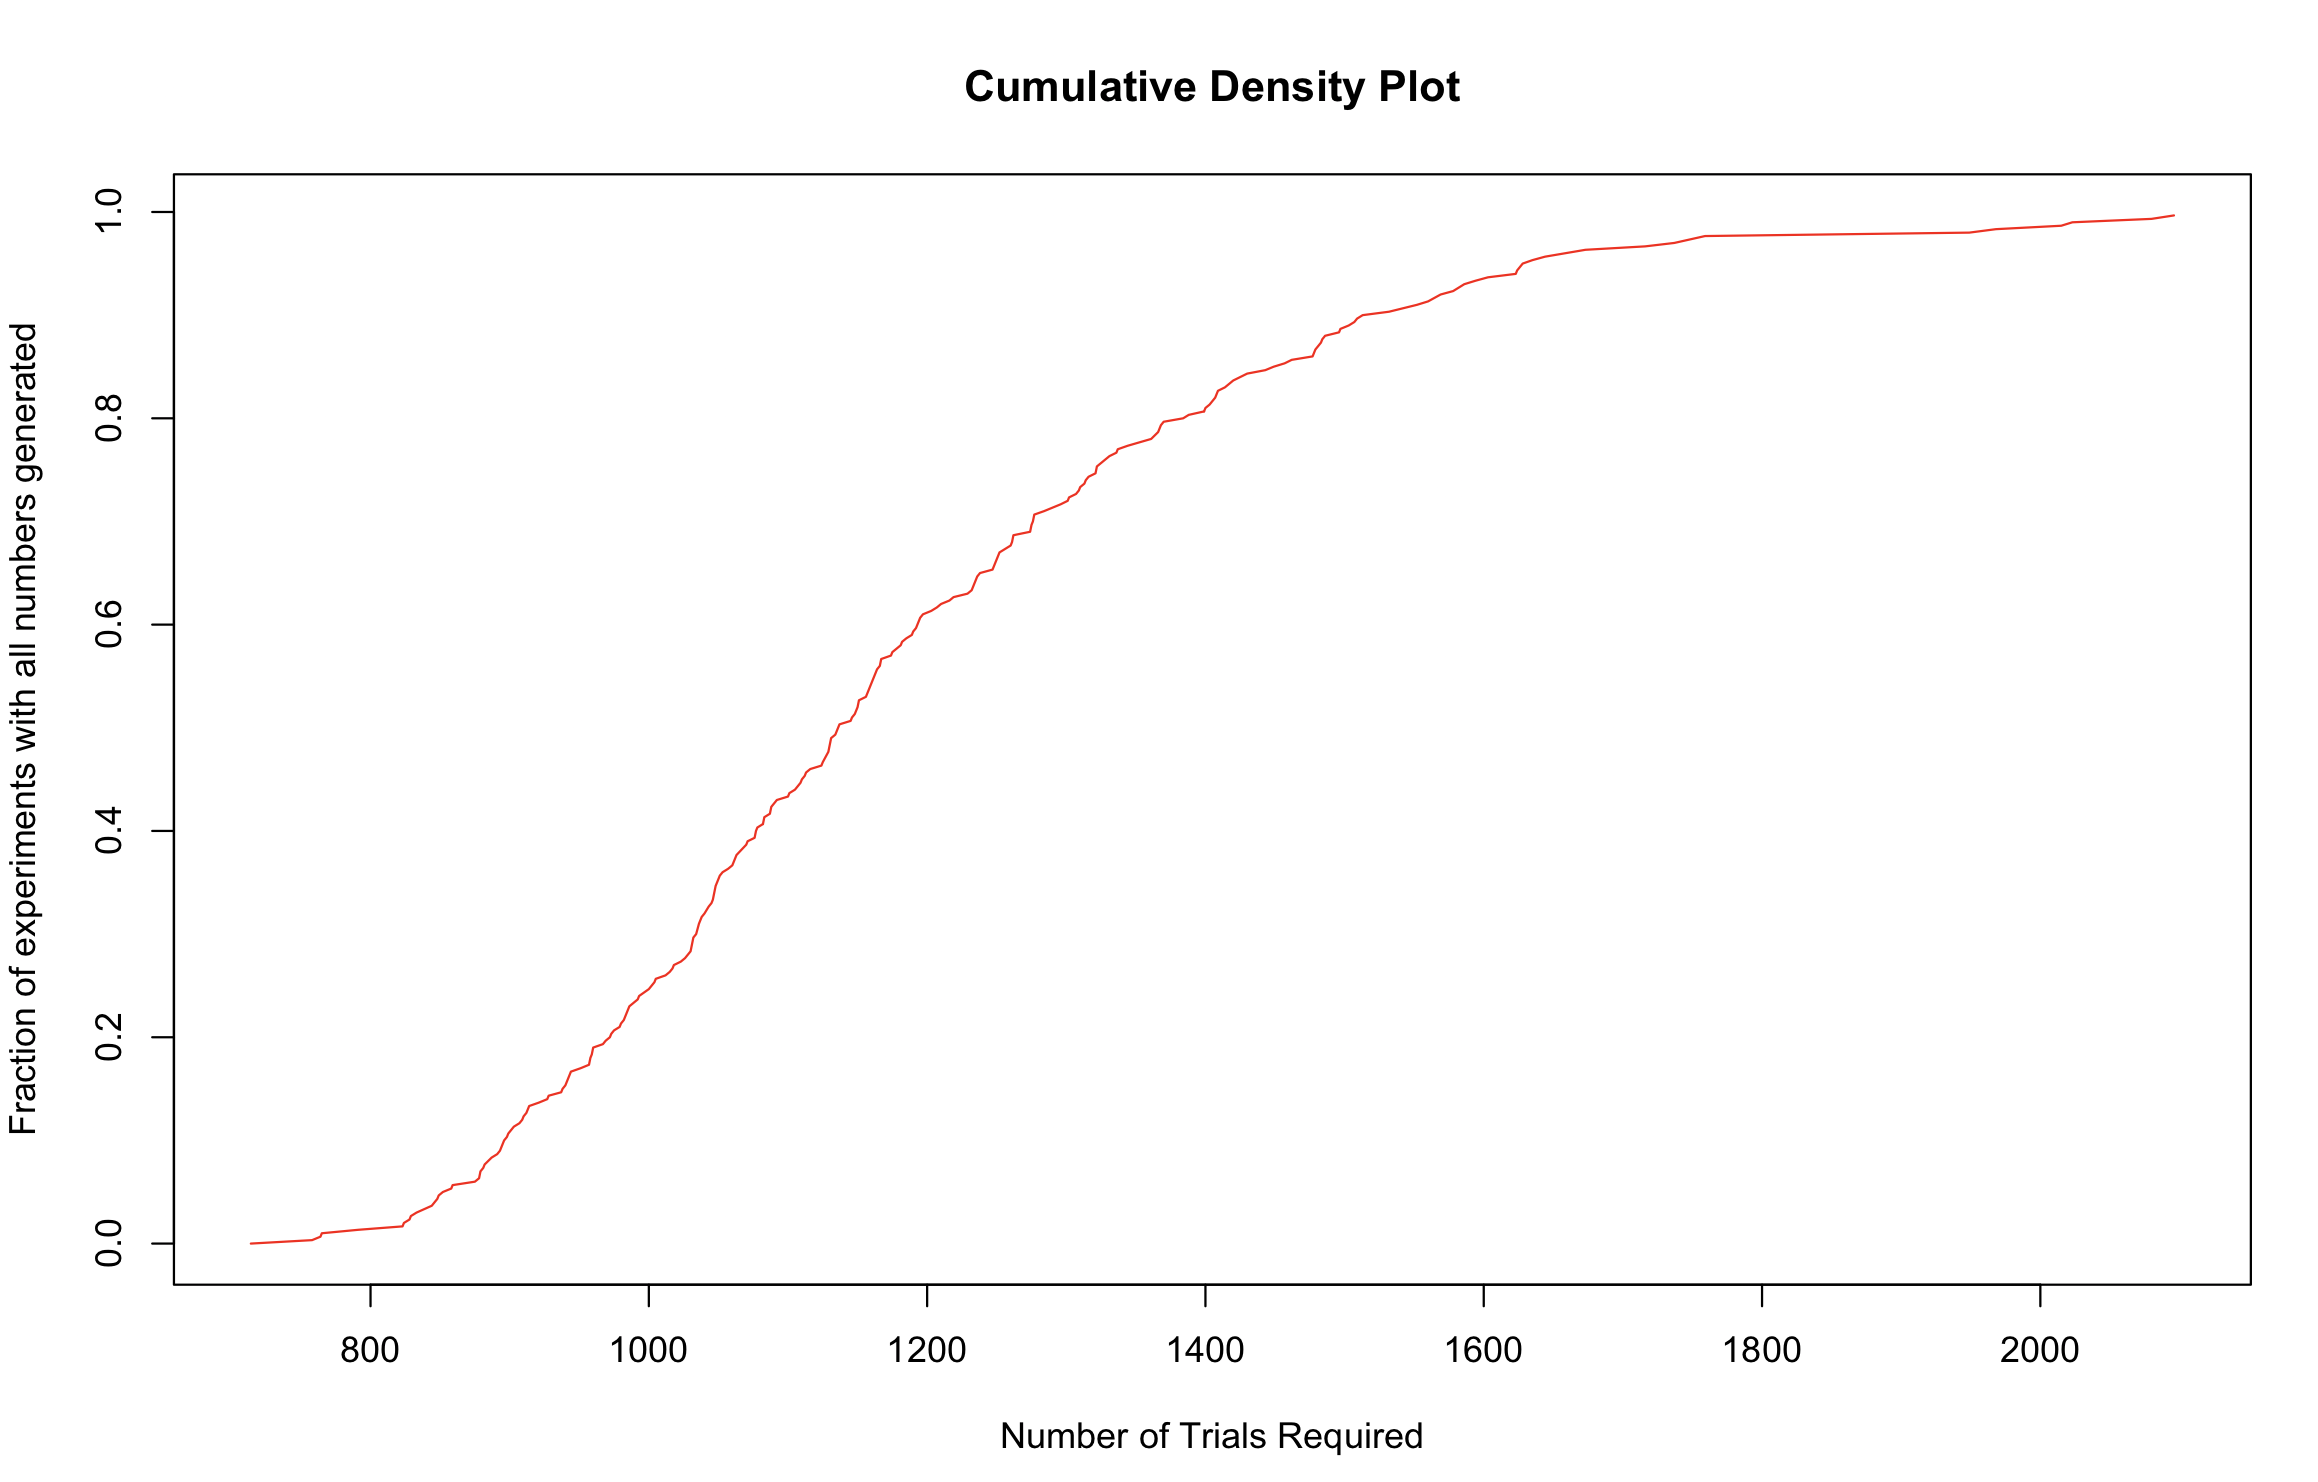
\includegraphics[width=5.5in]{figures/cumdenplot2b.png}
\caption{Cumulative density plot for trials till all numbers in domain are generated for experiment repeated $300$ times for a domain of size $4000$}
\label{cumplot2}
\end{figure}

\paragraph{C: (5 points)}
Use the above results to calculate the empirical expected value of $k$.\\

Empirical estimate for the expected number of random trials till all values are generated is $1191.0276$.

\paragraph{D: (10 points)} 
Describe how you implemented this experiment and how long it took for $n=200$ and $m=300$ trials.  \\

For each iteration of the experiment where it was run $m$ times, the number of trials till every number in the domain was generated, was recorded. The numbers of trials were put into an array and the array was sorted. For each entry in the array with index $x$, the corresponding fraction of experiments that succeeded in generating every number in the domain was computed as $\frac{x}{m}$.\\

For $300$ trials and domain size of $200$, it took $40$ $ms$ to run.\\

Show a plot of the run time as you gradually increase the parameters $n$ and $m$.  
(For at least 3 fixed values of $m$ between 300 and 5,000, plot the time as a function of $n$.)
You should be able to reach $n = 20{,}000$ and $m = 5{,}000$.  

The run time plot is shown in figure \ref{ccruntimes}.

\begin{figure}[!htb]
\centering
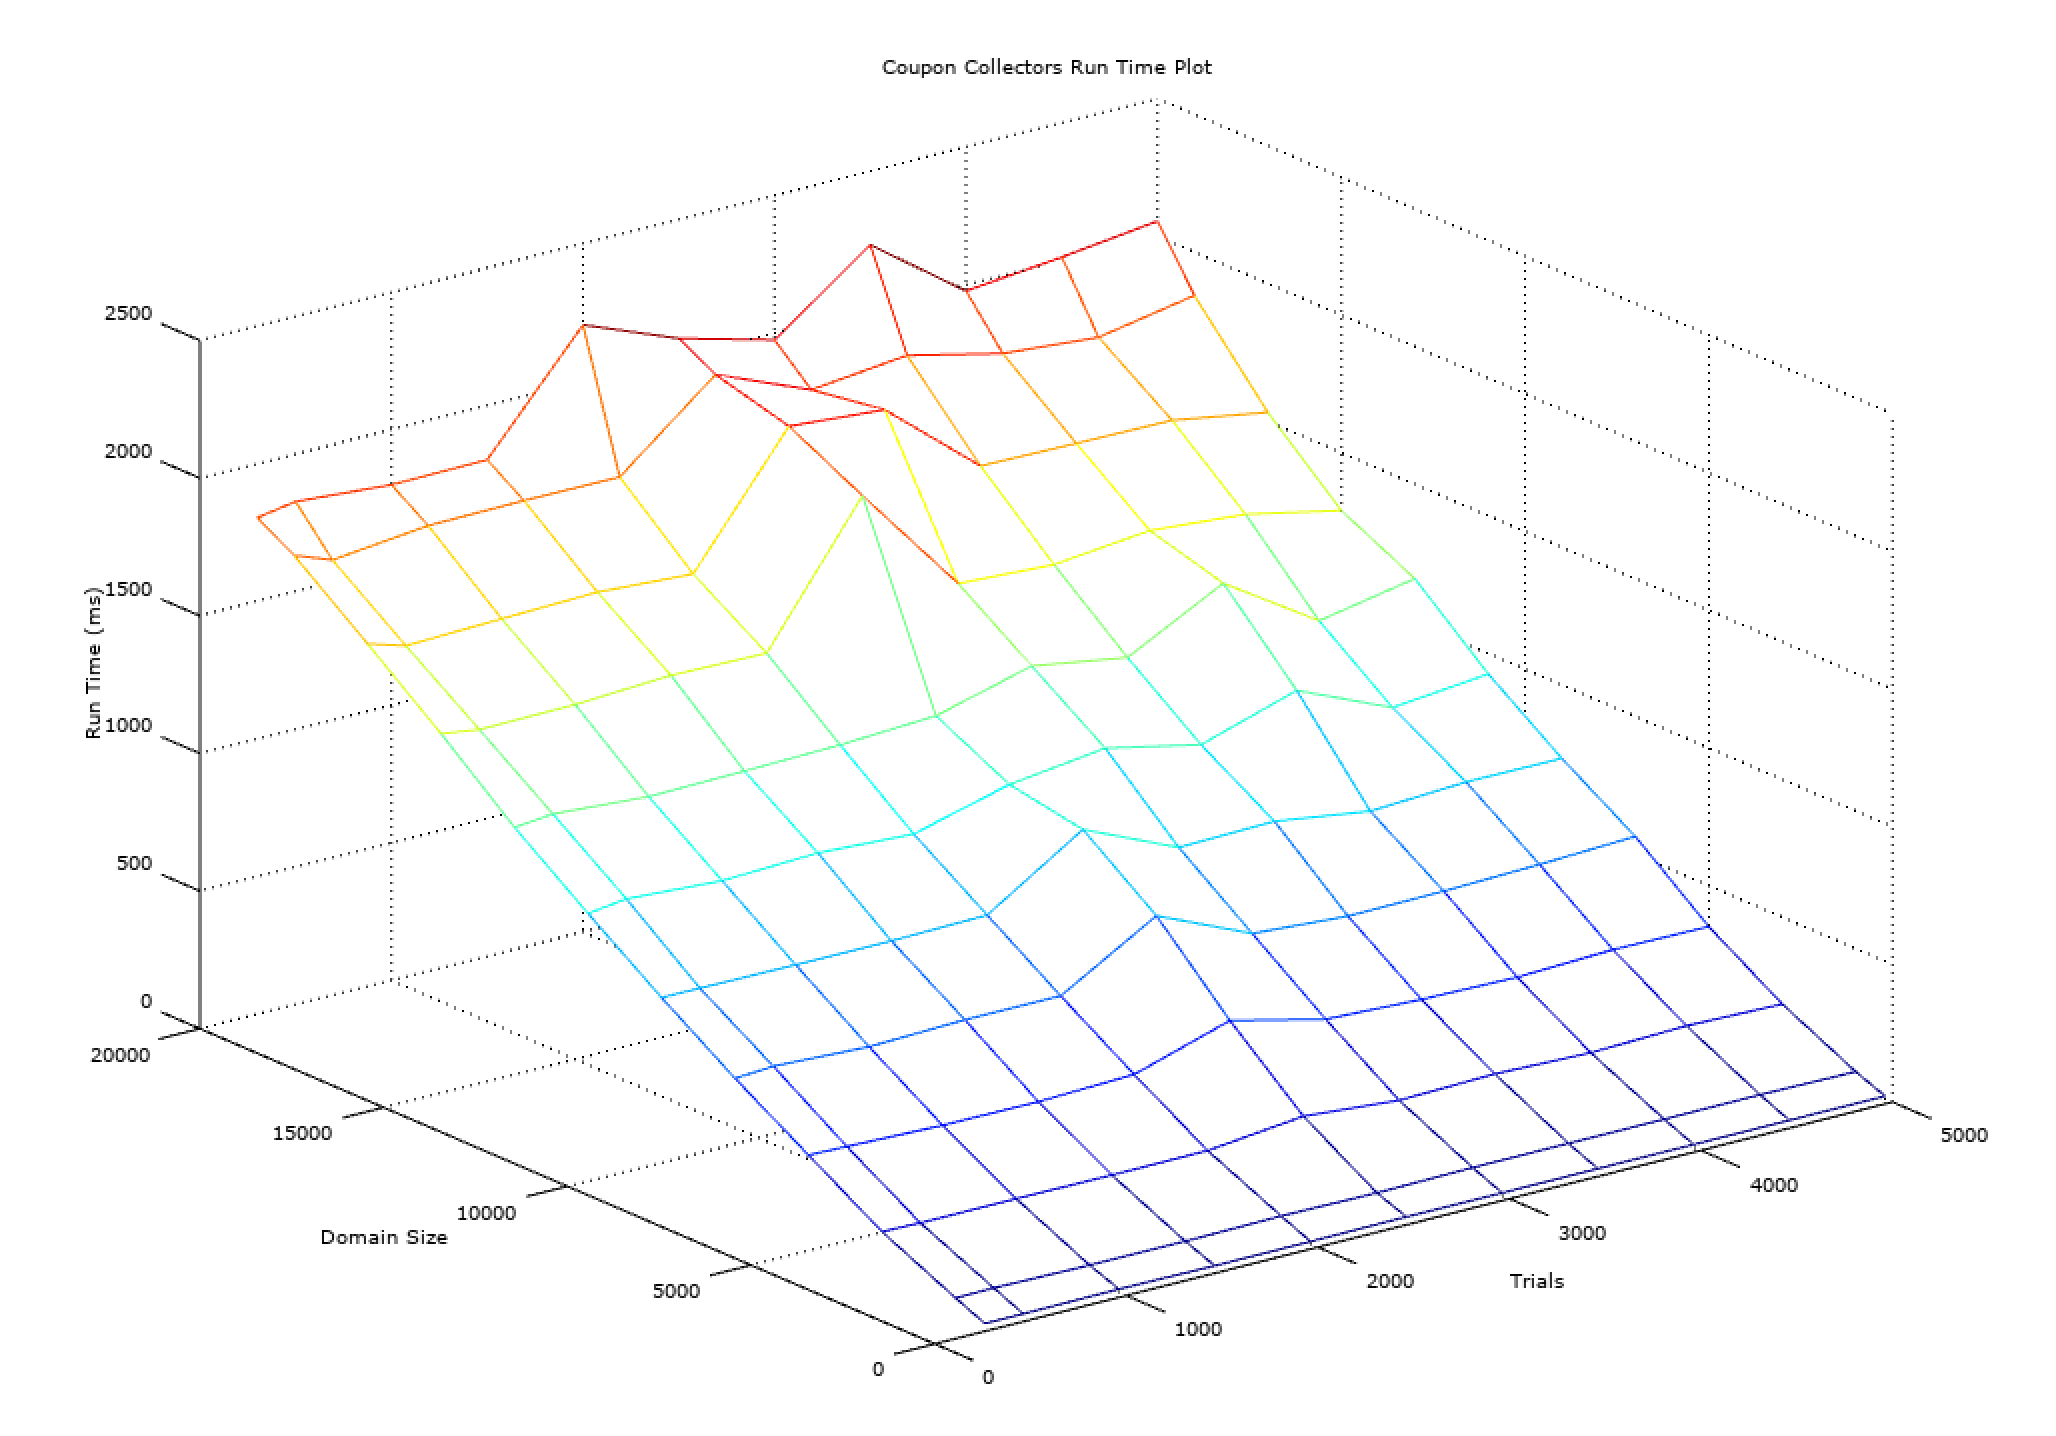
\includegraphics[width=5.5in]{figures/ccruntimes.png}
\caption{Coupon Collectors run time plot}
\label{ccruntimes}
\end{figure}
%%%%%%%%%%%%%%%%%%%%%%%%%%%%%%%%%%%%%%%%%%%%%%%%%%%%
%%%%%%%%%%%%%%%%%%%%%%%%%%%%%%%%%%%%%%%%%%%%%%%%%%%%
%%%%%%%%%%%%%%%%%%%%%%%%%%%%%%%%%%%%%%%%%%%%%%%%%%%%
\section{Comparing Experiments to Analysis (24 points)}

\paragraph{A: (12 points)}
Calculate analytically (using formulas from the notes in \textbf{L2}) the number of random trials needed so there is a collision with probability at least $0.5$ when the domain size is $n = 4000$.  There are a few formulas stated with varying degree of accuracy, you may use any of these -- the more accurate formula, the more sure you may be that your experimental part is verified, or is not (and you need to fix something).  
\\ \emph{[Show your work, including describing which formula you used.]}\\

The probability of a collision after $k$ trials is given by\\

\begin{equation*}
\begin{aligned}
\Pr(collision) &= 1 - \Pr(no \, collision)\\
&= 1 - \prod_{i=1}^{k-1} \frac{n-i}{n} 
\end{aligned}
\end{equation*}

By trial and error and running the computation in a program, I found out that for a domain size of $n=4000$, after $74$ trials, the probability of a collision is $0.4931$ and after $75$ trials the probability is $0.5025$. 

How does this compare to your results from \textsf{Q1.C}?  \\

In \textsf{Q1.C} the empirical result for expected number of trials till a collision was $86$ compared to the analytical result of $75$ trials for a collision probability of at least $0.5$.

\paragraph{B: (12 points)}
Calculate analytically (using formulas from the notes in \textbf{L2}) the expected number of random trials before all elements are witnessed in a domain of size $n=200$?  Again, there are a few formulas you may use -- the more accurate, the more confidence you might have in your experimental part.  
\\ \emph{[Show your work, including describing which formula you used.]}\\

The expected number of trials for seeing all $n$ elements is given by

\begin{equation*}
\begin{aligned}
T&= n \sum_{i=1}^n \frac{1}{i}
\end{aligned}
\end{equation*}

For a domain size of $n=200$, this was computed to be $1175$.\\

How does this compare to your results from \textsf{Q2.C}?\\

In \textsf{Q2.C} the empirical result for expected number of trials till for seeing all elements was $1192$ compared to the analytical result of $1175$ trials.

%%%%%%%%%%%%%%%%%%%%%%%%%%%%%%%%%%%%%%%%%%%%%%%%%%%%
%%%%%%%%%%%%%%%%%%%%%%%%%%%%%%%%%%%%%%%%%%%%%%%%%%%%
%%%%%%%%%%%%%%%%%%%%%%%%%%%%%%%%%%%%%%%%%%%%%%%%%%%%
\section{Random Numbers (16 points)}

Consider when the only random function you have is one that choses a bit at random.  In particular \texttt{rand-bit()} returns \texttt{0} or \texttt{1} at uniformly random.  

\paragraph{A: (6 points)}
How can you use this to create a random integer number between $1$ and $n=1024$?  \\

We can create an array of $1024$ booleans and each entry in the array can be set to $True$ or $False$ based on the value returned by \texttt{rand-bit()}. This array can be considered to be the binary representation of the random number that needs to be generated. Algorithm \ref{Rand1} is shown below that uses this technique for generating a random number when the upper limit is a power of $2$.\\

\begin{minipage}{\linewidth}
  \begin{algorithm}[H]
    \caption{Random Number Generation Algorithm}\label{Rand1}
    \begin{algorithmic}[1]
      \Procedure{Random Number Generation}{$upperLimit$}
        \State $exponent = \log_2 (upperLimit)$
      	\State $randomNumberArray$ = $boolean$[$exponent$]
	\For {$arrayIndex \, in \, range(1 \, to \, exponent)$}
	  \If {$\texttt{rand-bit()} == 0$}
	    \State $randomNumberArray [arrayIndex] = False$
	  \Else 
	    \State $randomNumberArray$ [$arrayIndex$] = $True$
	  \EndIf
	\EndFor
	\State $randomNumber = 1$
	\For {$arrayIndex \, in \, range(1 \, to \, exponent)$}
	  \If {$randomNumberArray [arrayIndex] == True$}
	    \State $randomNumber = randomNumber + 2^{arrayIndex - 1}$
	  \EndIf
	\EndFor
	\Return $randomNumber$
      \EndProcedure
    \end{algorithmic}
  \end{algorithm}
\end{minipage}\\

\paragraph{B: (5 points)}
Describe a Las Vegas randomized algorithm (``Las Vegas'' randomized algorithm means: it may run forever, but you can bound how long you expect it to take, and when it finishes you know it is done and correct) for generating a random number in $[n]$ when $n=1000$.  \\

Algorithm \ref{Rand2} shows a Las Vegas algorithm for generating a random number. When the upper limit for the random number is not a power of $2$, as in this case, the binary representation of the random number has a size such that the maximum number that can be generated, is larger than the upper limit. So in case that the random number generated is larger than the upper limit, the process is repeated till the generated random number is within the upper limit. Due to this reason, there is the possibility that the process may run forever.\\

In each run, the probability of generating a number within the upper limit of $1000$ is $\frac{1000}{1024}$ and the probability of failure is $\frac{24}{1024}$. So the $while$ loop in algorithm \ref{Rand2} is expected to have $\ceil*{\frac{1024}{1000}} = 2$ iterations.

\begin{minipage}{\linewidth}
  \begin{algorithm}[H]
    \caption{Las Vegas Random Number Generation Algorithm}\label{Rand2}
    \begin{algorithmic}[1]
      \Procedure{Las Vegas Random Number Generation}{$upperLimit$}
        \State $exponent = \ceil*{\log_2 (upperLimit)}$
	\State $randomNumberGenerated = False$
	\While {$not \, randomNumberGenerated$} 
      	  \State $randomNumberArray$ = $boolean$[$exponent$]
	  \For {$arrayIndex \, in \, range(1 \, to \, exponent)$}
	    \If {$\texttt{rand-bit()} == 0$}
	      \State $randomNumberArray [arrayIndex] = False$
	    \Else 
	      \State $randomNumberArray$ [$arrayIndex$] = $True$
	    \EndIf
	  \EndFor
	  \State $randomNumber = 1$
	  \For {$arrayIndex \, in \, range(1 \, to \, exponent)$}
	    \If {$randomNumberArray [arrayIndex] == True$}
	      \State $randomNumber = randomNumber + 2^{arrayIndex - 1}$
	    \EndIf
  	  \EndFor
	\If {$randomNumber \leq upperLimit$}
	  \State $randomNumberGenerated = True$
	\EndIf
	\EndWhile
	\Return $randomNumber$
      \EndProcedure
    \end{algorithmic}
  \end{algorithm}
\end{minipage}\\

\paragraph{C: (5 points)}  
Describe how many \texttt{rand-bit()} calls does the above procedure (extending your algorithm in \textbf{4B}) take as a function of $n$ (say I were to increase the value $n$, how does the number of calls to \texttt{rand-bit()} change)?  

\emph{[Keep in mind that in many settings generating a random bit is much more expensive that a standard CPU operation (like an addition, if statement, or a memory reference), so it is critical to minimize them.  ]}\\

In the above case where $n = 1000$, \texttt{rand-bit()} will be called $10$ times per iteration of the $while$ loop. The $while$ loop is expected to have $2$ iterations as described above. Hence we can expect 20 calls to be made to \texttt{rand-bit()}. This expected number of calls will not change till $n$ is increased till $1023$. When $n=1024$, the $while$ loop will execute only once as the random number generated will be at most $1024$. \\

When $n$ is $1025$, the binary number used for random number generation will have $11$ bits and the largest number that can be generated is $2048$. The probability of success becomes $\frac{1025}{2048}$ and that of failure becomes $\frac{1023}{2048}$. We can expect to call \texttt{rand-bit()} $11 \times 2 = 22$ times.\\

The number of calls $N$ to \texttt{rand-bit()} as a function of $n$ will be

\begin{equation*}
\begin{aligned}
N &= \ceil*{\log_2 {n}} \times 2
\end{aligned}
\end{equation*}

\vspace{-.1in}
%%%%%%%%%%%%%%%%%%%%%%%%%%%%%%%%%%%%%%%%%%%%%%%%%%%%
%%%%%%%%%%%%%%%%%%%%%%%%%%%%%%%%%%%%%%%%%%%%%%%%%%%%
%%%%%%%%%%%%%%%%%%%%%%%%%%%%%%%%%%%%%%%%%%%%%%%%%%%%
\section{BONUS : PAC Bounds (2 points)}

Consider a domain size $n$ and let $k$ be the number of random trials run, where each trial obtains each value $i \in [n]$ with probability $1/n$.  
Let $f_i$ denote the number of trials that have value $i$.  
Note that for each $i \in [n]$ we have $\E[f_i] = k/n$.  
Let $\mu = \max_{i \in [n]} f_i/k$.  

Consider some parameter $\delta \in (0,1)$.  
As a function of parameter $\delta$, how large does $k$ need to be for 
$\Pr[ |\mu - 1/n| \geq 0.01] \leq \delta$?
That is, how large does $k$ need to be for \emph{all} counts to be within $1\%$ of the average with probability $\delta$? 
\emph{(Fine print:  you don't need to calculate this exactly, but describe a bound as a function of $\delta$ for the value $k$ which satisfies PAC property.  Notes here should help: \url{http://www.cs.utah.edu/~jeffp/teaching/cs5140/L2+Chern-Hoeff.pdf})}

How does this change if we want
$\Pr[ |\mu - 1/n| \geq 0.001] \leq \delta$ (for $0.1\%$ accuracy)?

\emph{[Make sure to show your work.]}

\end{document}
